\documentclass[UTF8,a4paper,12pt]{ctexart}
\usepackage{amsmath}
\usepackage{geometry}
\usepackage{graphicx}
\usepackage{epstopdf}
\usepackage{booktabs}
\usepackage{listings}
\usepackage{array}
\usepackage{amssymb}
\usepackage{amsmath}
\usepackage{pdfpages}
\usepackage{tikz}
\usepackage{float}
\usepackage{fancyhdr}
\usepackage[section]{placeins}
\usepackage{titlesec}
\usepackage{titletoc}
\usepackage{setspace}
\usepackage[hidelinks]{hyperref}
\linespread{1.375}
\setmainfont{Times New Roman}
\ctexset{
	section={
		format=\bfseries \zihao{3} \heiti \centering,
		name={第,章},
		number=\chinese{section},
	},
	subsection={
		format=\bfseries \zihao{4} \heiti,
	},
	subsubsection={
		format=\bfseries \zihao{-4},
	}
}
\titlecontents{section}
	[3cm]
	{\zihao{4}}
	{\contentslabel{3cm}\hspace{-1.1cm}}
	{\hspace{-3cm}}
	{~\titlerule*[0.7pc]{$.$}~\contentspage}


\renewcommand{\contentsname}{\fontsize{16pt}{\baselineskip}\heiti 目  录}
%这段注释是留给画流程图用的
%\usetikzlibrary{shapes,arrows}
%\tikzstyle{startstop} = [rectangle,rounded corners, minimum width=3cm,minimum height=1cm,text centered,draw=black, fill=red!10]
%\tikzstyle{io} = [trapezium, trapezium left angle = 70,trapezium right angle=110,minimum width=3cm,minimum height=1cm,text centered,draw=black, fill=green!10]
%\tikzstyle{process} = [rectangle,minimum width=3cm,minimum height=1cm,text centered,draw=black, fill=blue!10]
%\tikzstyle{processsmall} = [rectangle,minimum width=3cm,minimum height=1cm,text centered,text width=3cm,draw=black, fill=blue!10]
%\tikzstyle{decision} = [diamond,minimum width=3cm,minimum height=1cm,text centered, text width=3cm,draw=black, fill=orange!10]
%\tikzstyle{arrow} = [thick,->,>=stealth]
\geometry{left=3cm,right=2.5cm,top=3cm,bottom=2.5cm}
\pagestyle{fancy}
\fancyhf{}
\fancyhead[C]{\fontsize{9pt}{\baselineskip} 安徽农业大学本科毕业论文(设计)} 


%没有使用标题生成,有点小问题好像
%\title{\textbf{\fontsize{36pt}{\baselineskip}本科生毕业论文(设计)\vspace{-2cm}}}
%\date{}
\begin{document}
	\vspace{5cm}
	\begin{figure}[!h]
		\centering
		
\includegraphics[width=0.8\textwidth]{pic/校徽.pdf}
		\label{fig0}
	\end{figure}
	%\maketitle
	\textbf{\fontsize{36pt}{\baselineskip}本科生毕业论文(设计)}
	\vspace{3cm}
	\begin{table}[!h]
		\centering
		\renewcommand\arraystretch{2}
		\setlength\tabcolsep{22pt}%调整观感
		\begin{tabular}{cccc}
			%自己补充关键内容
			\textbf{\heiti\zihao{4} 题  目:} &\multicolumn{3}{c}{\zihao{4}基于1234567890的管理系统} \\ 
			\cline{2-4}
			\textbf{\heiti\zihao{4} 姓  名: }&\multicolumn{3}{c}{\zihao{4}禾斗匕匕}\\ 
			\cline{2-4}
			\textbf{\heiti\zihao{4} 学  号: }&\multicolumn{3}{c}{\zihao{4}20123456}\\ 
			\cline{2-4}
			\textbf{\heiti\zihao{4} 学  院: }&\multicolumn{3}{c}{\zihao{4}信息与人工智能学院} \\ 
			\cline{2-4}
			\textbf{\heiti\zihao{4} 专  业: }&\multicolumn{3}{c}{\zihao{4}计算机科学与技术} \\
			\cline{2-4}
			\textbf{\heiti\zihao{4} 指导教师:}&\zihao{4} 佐巴扬 &\textbf{\heiti\zihao{4} 职  称:}&\zihao{4} 机 长 \\
			\cline{2-2} \cline{4-4}
		\end{tabular}
	\end{table}

	\vspace{4cm} 
	\begin{table}[!h]
		\renewcommand\arraystretch{2}
		\setlength\tabcolsep{16pt}
		\centering
		\begin{tabular}{c}
			\textbf{\fontsize{16pt}{\baselineskip}\heiti 中 国 • 合 肥 }\\
			\textbf{\fontsize{16pt}{\baselineskip}\heiti 二 〇 二 四 年 五 月} \\
			% 0 0 日
		\end{tabular}
	\end{table}
	%\centerline{\textbf{\fontsize{16pt}{\baselineskip}\heiti 中 国 • 合 肥}}
	%\vspace{1cm}
	%\centerline{\textbf{\fontsize{16pt}{\baselineskip}\heiti 2 0 2 4 年 5 月 0 0 日}}
	\thispagestyle{empty}
	\newpage 
	\vspace{1cm} \par \textbf{\fontsize{18pt}{\baselineskip}\heiti 安徽农业大学本科生毕业论文(设计)原创性声明}
	\vspace{1cm} \par 本人郑重声明:所呈交的毕业论文(设计),是本人在导师的指导下,独立进行研究工作所取得的成果。除文中已经注明引用的内容外,本论文不包含任何其他个人或集体已经发表或撰写过的作品成果。对本文的研究做出重要贡献的个人和集体,均已在文中以明确方式标明。本人完全意识到本声明的法律结果由本人承担。
	\vspace{1cm} \par 论文作者签名:            日期:    年  月  日
	\vspace{6cm} \par \textbf{\fontsize{18pt}{\baselineskip}\heiti  安徽农业大学本科生毕业论文(设计)使用授权声明}
	\vspace{1cm} \par 本学位论文作者完全了解学校有关保留、使用毕业论文(设计)的规定,同意学校保留并向国家有关部门或机构送交论文的复印件和电子版,允许论文被查阅和借阅。本人授权安徽农业大学教务处可以将本毕业论文(设计)的全部或部分内容编入有关数据库进行检索,可以采用影印、缩印或扫描等复制手段保存和汇编毕业论文(设计)。
	\vspace{1cm} \par 论文作者签名:            导师签名:
	\vspace{0.5cm} \par 日期:    年  月  日     日期:    年  月  日
	\thispagestyle{empty}
	
	\newpage
	
	\begin{spacing}{1.4}
	%目录上面的行间距自己调整一下,尽量不要超过一页目录,否则要设置第二页页面格式为empty。
	\tableofcontents
	
	\end{spacing}
	\thispagestyle{fancy}
	\fancyfoot{}
	\newpage
	\fancyfoot[C]{\thepage} 
	\addcontentsline{toc}{section}{摘  要} \tolerance=500
	\centerline{\textbf{\fontsize{16pt}{\baselineskip}\heiti 摘  要}}
	\vspace{0.4cm}
	%距离这个东西自己看着调整,我觉得这样调整后好看
	111111不中嘞哥。..点击目录或引用实现跳转哥。。

	\vspace{0.2cm}
	\par \textbf{\fontsize{14pt}{\baselineskip}\heiti 关键词: }123
	\setcounter{page}{1}
	\pagenumbering{Roman}
	\newpage
	\addcontentsline{toc}{section}{ABSTRACT}\tolerance=500
	\centerline{\textbf{\large ABSTRACT}}
	\vspace{0.4cm}
	111111英文摘要找GPT4帮你翻译U know M3
	\vspace{0.4cm}
	\par \textbf{\fontsize{14pt}{\baselineskip}KEYWORDS: }123
	\newpage
	\setcounter{page}{1}
	\pagenumbering{arabic}
	\section{绪论}
	\subsection{研究背景及意义}
	下面的东西自己修改,标题也是,我这是示例标题\footnote{我也不知道为什么}
	
	\subsection{论文的主要研究内容及其组织结构}
	扣1111111送地狱火
	
	\section{理论基础}
	
	\subsection{某理论基础某理论基础}
	\begin{equation}
		\begin{array}{c}
			\text {deg  = }\left\{\begin{array}{lc}
				\arctan (\frac{y-y_{0}}{x-x_{0}}) & (x\ge 0,y\ge 0) \\
				\arctan (\frac{y-y_{0}}{x-x_{0}})+\pi & (x<  0,y\ge 0) \\
				\arctan (\frac{y-y_{0}}{x-x_{0}})+\pi & (x\ge 0,y<  0) \\
				\arctan (\frac{y-y_{0}}{x-x_{0}})+2\pi & (x<  0,y<  0) \\
			\end{array}\right.
		\end{array}
	\end{equation}
	公式示例0  \ \  我也不知道什么公式

	
	\begin{table}[htp]
		\renewcommand\arraystretch{1.6}
		\setlength\tabcolsep{20pt}
		\centering
		\begin{center}
			\fontsize{11pt}{\baselineskip}\heiti 表1  \ \  表格坐标示例 \par Table 1. \ \ Table axis template
		\end{center} 
		\vspace{-0.4cm} 
		\begin{tabular}{cccc}
			\toprule
			起始边x坐标&起始边y坐标&终边x坐标&终边y坐标\\
			\midrule
			1&782&0&762\\
			1&782&1&762\\
			1&782&0&763\\
			...&...&...&...\\
			0&948&4&939\\
			0&950&4&939\\
			0&951&4&939\\
			...&...&...&...\\
			\bottomrule
		\end{tabular}
		\vspace{-0.4cm} 
	\end{table}
	
	\subsubsection{某理论基础详细介绍}
	首先设置$(x_{0j},y_{0j}) = \{(x_i,y_i)|x_{0j}=\min x_i,y_{0j}=\min y_i\}$为初始点,并设置其三个扇区角度为:
	$(\alpha ,\beta ,\gamma) = (0,\frac{2\pi}{3} ,\frac{4\pi}{3} )$ 。\textsuperscript{\cite{Ref1}}
	\begin{equation}
		\begin{array}{c}
			\text {}\left\{\begin{array}{l}
				y=\frac{a}{x^2}\\
				O(y) = y^2\times x\\
				z=(\frac{\max(x)}{x})^2
			\end{array}\right.
		\end{array}
	\end{equation}
	

	\section{技术介绍}
	\subsection{某技术详细介绍}
	6666666\textsuperscript{\cite{Ref3}}
	\begin{figure}[!h]
		\centering
		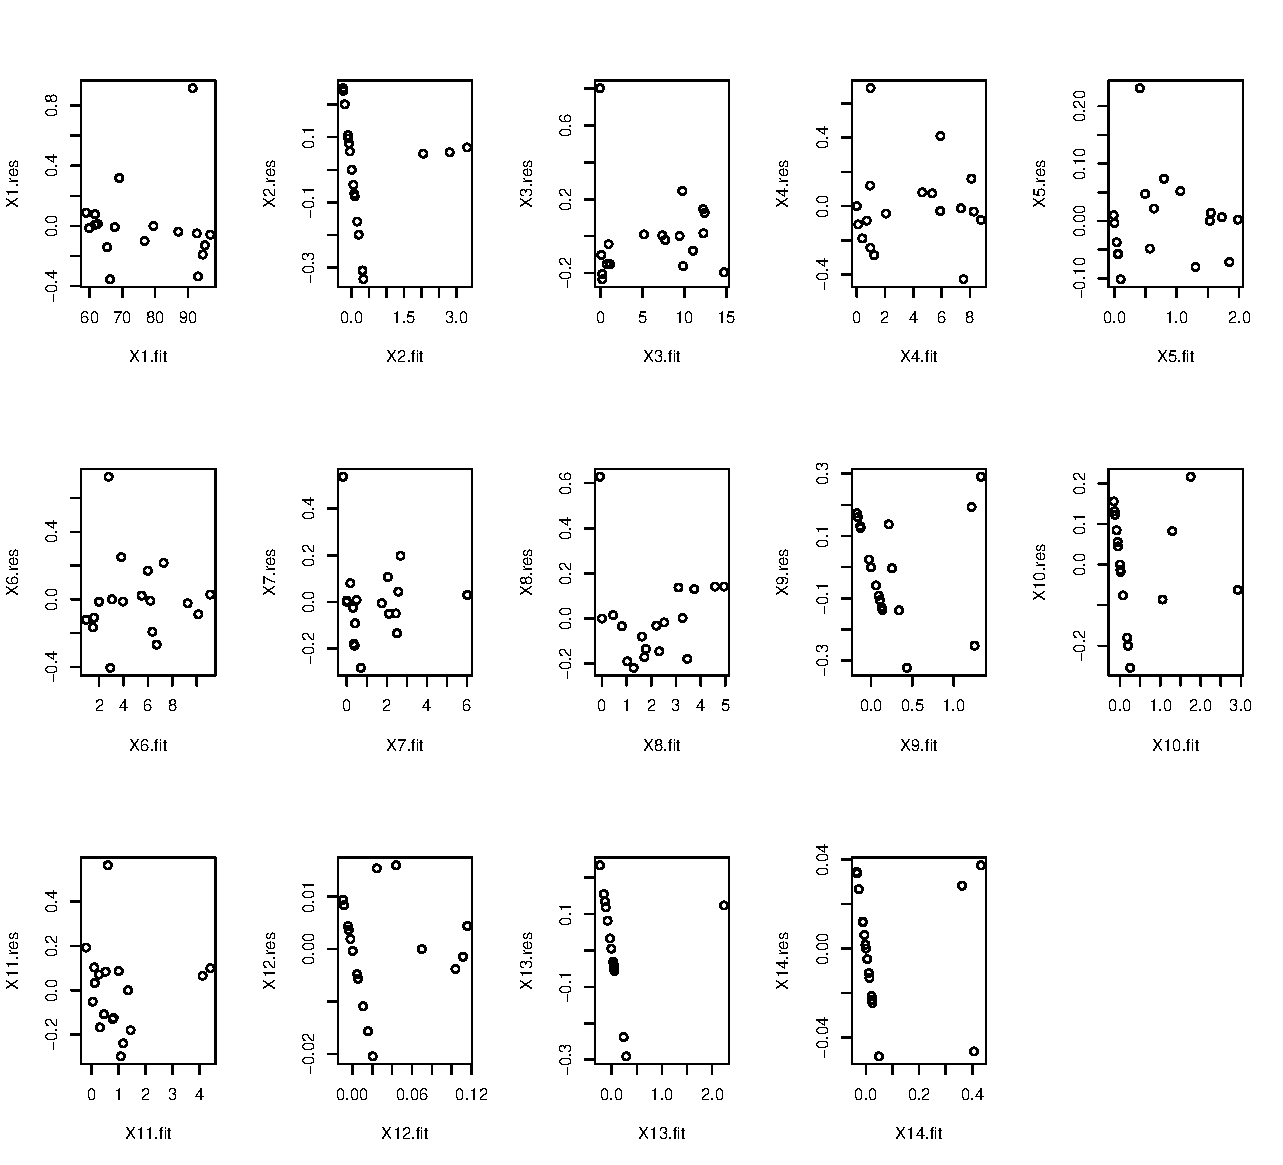
\includegraphics[width=0.8\textwidth]{pic/cti.pdf}
		\label{tu}
	\end{figure}
	\vspace{-0.5cm}
	\begin{center}
		\fontsize{11pt}{\baselineskip}\heiti 图2 \ \  数据对比 \par Figure 2. \ \ Data compare
	\end{center} 
	
	\section{架构实现}
	\subsection{某架构详细实现}
	网恋被骗8000块\textsuperscript{\cite{Ref2}}
	\begin{equation}
		\begin{array}{c}
			\min cost  =10 \sum_{i=1} m_{i}+\sum_{i=1} n_{i}  \\
			\text { s. t. }\left\{\begin{array}{l}
				\sum_{i, j=1}^{n} W_{j} \times n_{i}+\sum_{i=1, j=1}^{m} W_{j} \times n_{i} \geq  \sum_{j=1}^{} W_{j} \times 90\% \\
				m_{i}=0,1  \\ 
				n_{i}=0,1  \\
				\sqrt{\left(x-x_{0j}\right)^{2}-\left(y-y_{0j}\right)^{2}} \leq 30=H o n g(x, y) \\
				\sqrt{\left(x-x_{0j}\right)^{2}-\left(y-y_{0j}\right)^{2}} \leq 10=\operatorname{Wei}(x, y)\\
			\end{array}\right.
		\end{array}
	\end{equation}
	什么垃圾规划

	\section{总结与展望}
	哎,安农专给的word模版就是一坨答辩,按下tab的瞬间整个word都变了
	
	\begin{figure}[h]
		\vspace{-0.1cm} 
		\begin{minipage}[t]{0.45\linewidth}
			\centering
			
\includegraphics[height=6cm,width=7cm]{pic/fknumscom-eps-converted-to.pdf}
			
			\begin{center}
				\fontsize{11pt}{\baselineskip}\heiti 图3(a) \ \  哈里路大炫风! \par Figure 3(a). \ \ Aolianfei Allin
			\end{center} 
		\end{minipage}
		\begin{minipage}[t]{0.45\linewidth}
			\centering
			
\includegraphics[height=6cm,width=7cm]{pic/fknumstime-eps-converted-to.pdf}
			
			\begin{center}
				\fontsize{11pt}{\baselineskip}\heiti 图3(b)  \ \  我的图图呢  \par Figure 3(b). \ \ Where is 图图
			\end{center} 
		\end{minipage}
	\end{figure}
	\newpage
	\addcontentsline{toc}{section}{参考文献} \tolerance=500
	\centerline{\textbf{\fontsize{16pt}{\baselineskip}\heiti 参考文献}}
	\small
	%我这个参考文献的模版好像有点问题,但是也不是不能用
	\vspace{-0.5cm} 
	\renewcommand{\refname}{\leftline{Reference}}
	\begin{thebibliography}{}
		\vspace{-1cm} 
		\bibitem{Ref1}
		安徽农业大学信息与人工智能学院荣誉出品:D
		\bibitem{Ref2}
		大香蕉一条大香蕉,你的感觉真的很奇妙~~~
		\bibitem{Ref3}
		这个入开桂了
	\end{thebibliography}

	\newpage
	\addcontentsline{toc}{section}{致  谢} \tolerance=500
	\centerline{\textbf{\fontsize{16pt}{\baselineskip}\heiti 致  谢}}
	\normalsize
	\vspace{0.4cm}
	我测,不会真有人用农专发的唐氏模版吧
	\newpage
	\pagestyle{empty}
	\addcontentsline{toc}{section}{附  录} \tolerance=500
	\centerline{\textbf{\fontsize{16pt}{\baselineskip}\heiti 附  录}}
	\begin{spacing}{1.1}
	\begin{verbatim}
	感谢你使用此模版!
		
	\end{verbatim}
	\end{spacing}
	
	
\end{document}